\section{マージン最大化分類}
導入では、サポートベクターマシンの基本的な考え方は超平面を用いて与えられたデータを分類することだと述べた。ここではその具体的な操作を見ていくものとする。

話を具体化するために2次元におけるクラス分類を用いて説明する。以下の図のデータセットは線分によってクラス分類できることは直感的にわかる。その際に、線分の方程式は以下のようとなる。
\begin{figure}[h]
  \centering
  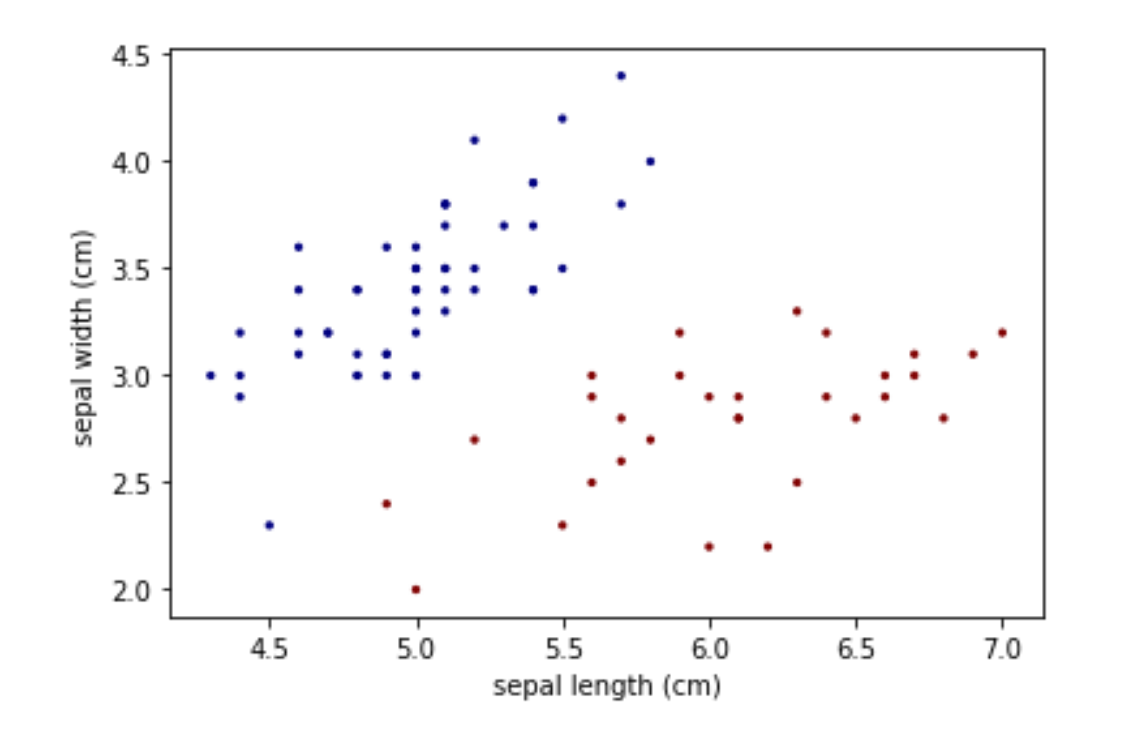
\includegraphics[width=5cm]{figure/section1/figure1.png}
  \caption{直線により分類できるデータセット}
\end{figure}
\begin{equation}
  w_1x_1 + w_2x_2 + c = 0
\end{equation}

この式はベクトル表記を用いて以下のように表現できる。
\begin{equation}
  \bm{w}^{\mathrm{T}}\bm{x} + \gamma = 0
\end{equation}

ただし、
\bm{w} = 
\begin{pmatrix}
  w_1 \\
  w_2 \\
\end{pmatrix}
,
\bm{x} = 
\begin{pmatrix}
  x_1 \\
  x_2 \\
\end{pmatrix}
,
\gamma \in \mathbb{R}

この線分より上に存在する点$\bm{x_+}$について$\bm{w}^{\mathrm{T}}\bm{x_+} + \gamma > 0$、下に存在する点$\bm{x_-}$について$\bm{w}^{\mathrm{T}}\bm{x_-} + \gamma < 0$が成立することがわかる。
\begin{figure}[h]
  \centering
  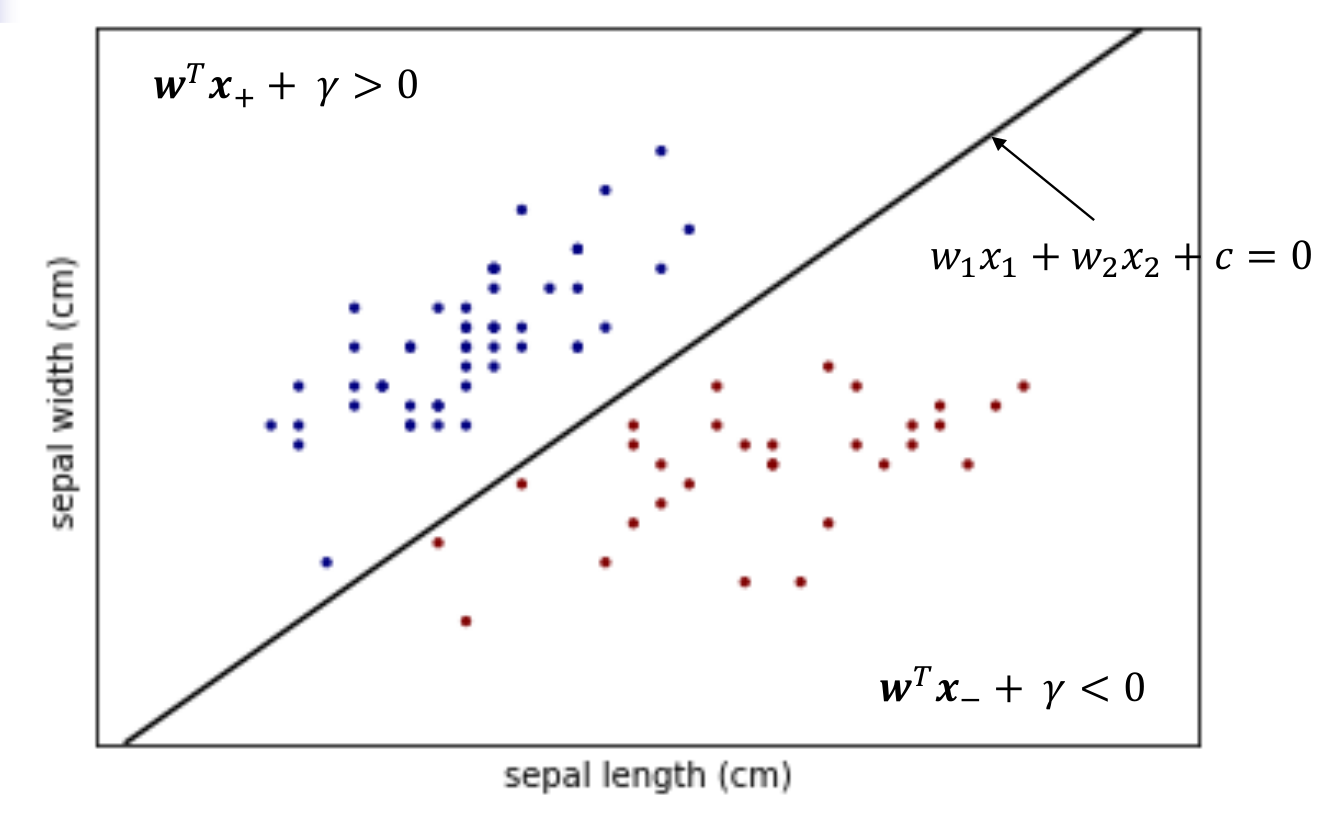
\includegraphics[width=5cm]{figure/section1/figure4.png}
  \caption{境界線とサンプルの関係}
\end{figure}

ここで、サポートベクターマシンは教師あり学習であるので、データセット
${\it{D}} = \{\bm{x_i}, y_i\}$について、$y_i = +1$または$y_i = -1$というラベルが予め与えられているとすると、データ・セットの各点について以下の式が成立すれば正しいクラス分類ができたと言える。
\begin{equation}
  (\bm{w_i}^{\mathrm{T}}\bm{x_i} + \gamma)y_i > 0
\end{equation}

次に、マージンを定義することとする。マージンを$m_i$とし、
\begin{equation}
    m_i = (\bm{w_i}^{\mathrm{T}}\bm{x_i} + \gamma)y_i
 \end{equation}
と置く。マージンはデータセットが直線$\bm{w}^{\mathrm{T}}\bm{x} + \gamma$と最も距離が近い点の間隔のようなものと考えることができる。また、上述のような点は「サポートベクター」と呼ばれる。以後の計算はサポートベクターが直線$\bm{w}^{\mathrm{T}}\bm{x} + \gamma = 1$上にあると仮定して計算をしていくこととする。
\begin{figure}[h]
  \centering
  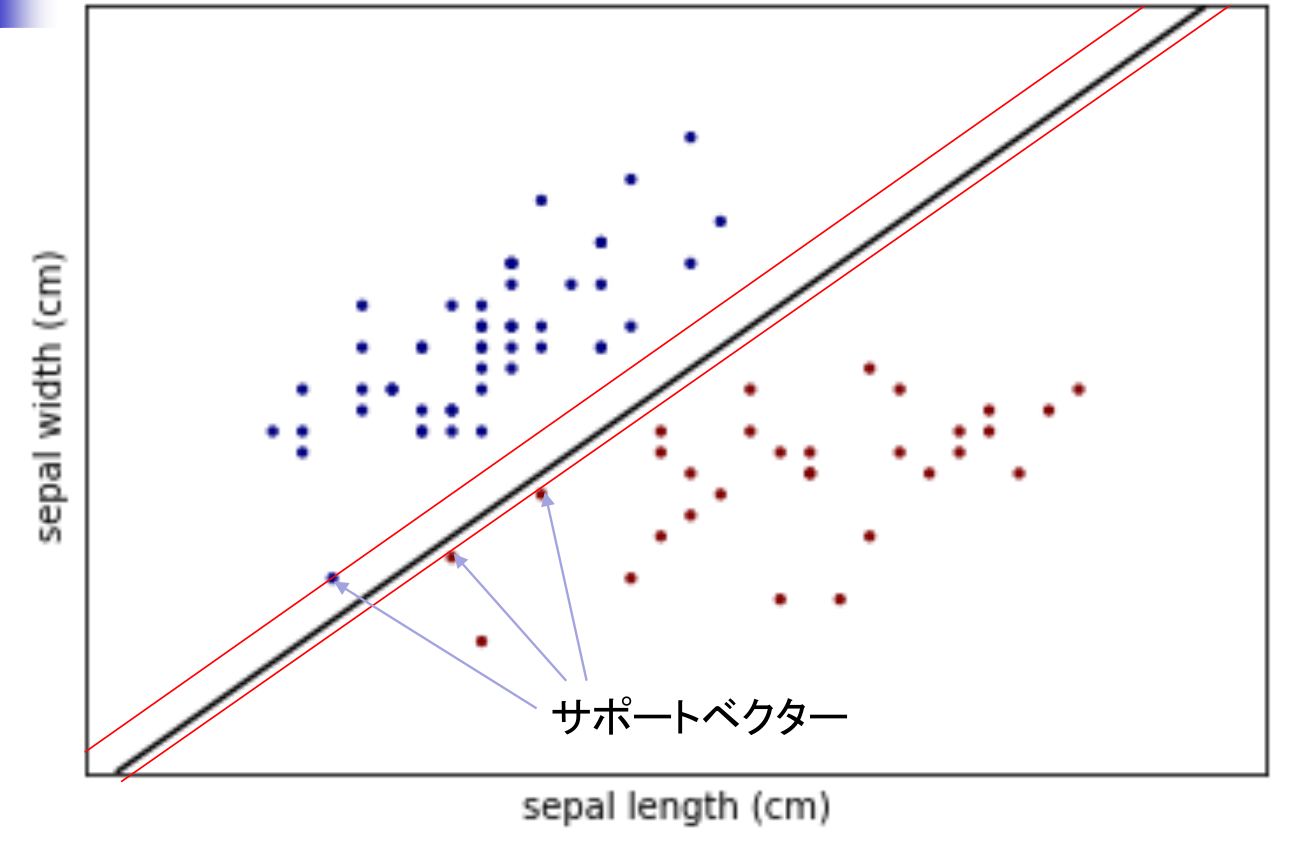
\includegraphics[width=5cm]{figure/section1/figure2.png}
  \caption{サポートベクター}
\end{figure}

サポートベクターが直線$(\bm{w}^{\mathrm{T}}\bm{x} + \gamma) = 1$上にあるとき、サポートベクターと直線$(\bm{w}^{\mathrm{T}}\bm{x} + \gamma) = 0$間の距離は以下の式によって計算される。
\begin{equation}
  \frac{(\bm{w}^{\mathrm{T}}\bm{x_i} + \gamma)y_i}{\|\bm{w}\|_2}
\end{equation}
サポートベクターが$\bm{w}^{\mathrm{T}}\bm{x_i} + \gamma = 1$上にあるとき、サポートベクターを含む各クラスのデータは$\bm{w}^{\mathrm{T}}\bm{x_i} + \gamma \ge 1$における領域にある。故に、
\begin{equation}
  \min\frac{\bm{w}^{\mathrm{T}}\bm{x_i} + \gamma}{\|\bm{w}\|_2} = \frac{1}{\|\bm{w}\|_2}
\end{equation}
$\frac{1}{\|\bm{w}\|_2}$はこのサポートベクターマシンのマージンの最小値である。しかし、サポートげクターマシンのマージンの最小値を最大化することにより、データ変動に強いサポートベクターマシンを作成できる。故に、
\begin{equation}
  \max\frac{1}{\|\bm{w}\|_2}\text{\ \ \ }{\it{s.t.}}\text{\ \ \ }\bm{w}^{\mathrm{T}}\bm{x_i} + \gamma \ge 1
\end{equation}
を求めれば最大マージンを計算できるが、この問題は以下の問題に同置である。
\begin{equation}
  \min\|\bm{w}\|_2\text{\ \ \ }{\it{s.t.}}\text{\ \ \ }\bm{w}^{\mathrm{T}}\bm{x_i} + \gamma \ge 1
\end{equation}
以上に仮定したサポートベクターマシンはサポートベクターを境界として必ず超平面を用いて与えられたサンプルを正しく分類できると仮定した。このようなものをハードマージン・サポートベクターマシンという。しかし、現実では与えられたサンプルは超平面によりきれいに分けることができないものが多い。その際に、マージンについての制限$(\bm{w}^{\mathrm{T}}\bm{x_i} + \gamma)y_i \ge 1$を緩めたものをソフトマージン・サポートベクターマシンという。
\begin{figure}[h]
  \centering
  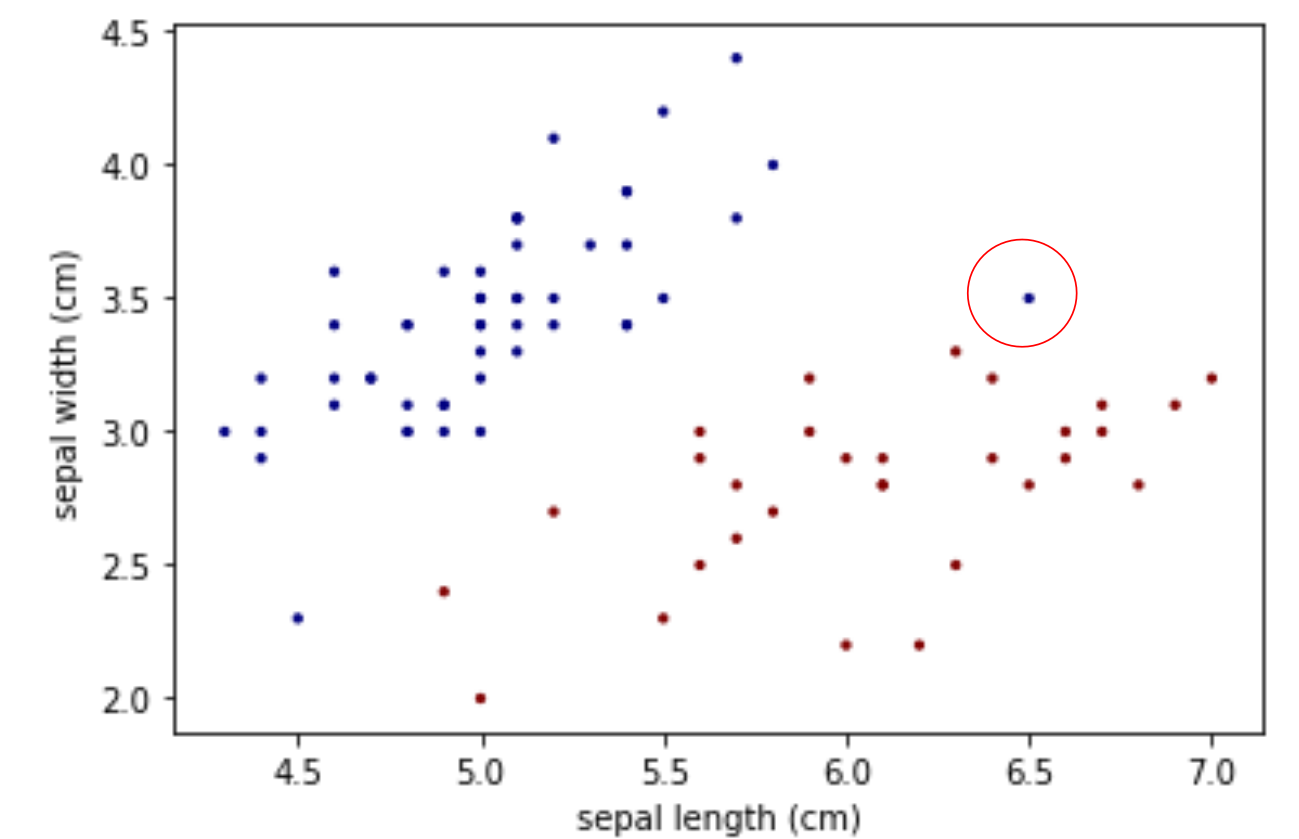
\includegraphics[width=5cm]{figure/section1/figure3.png}
  \caption{超平面によりサンプルを分類できない例}
\end{figure}
  



  




